In this lab we will perform a DoS attack on a Windows 10 virtual machine.
The attacker will be a Kali Linux virtual machine on the same 'host-only' network.

\begin{figure}[H]
    \centering
    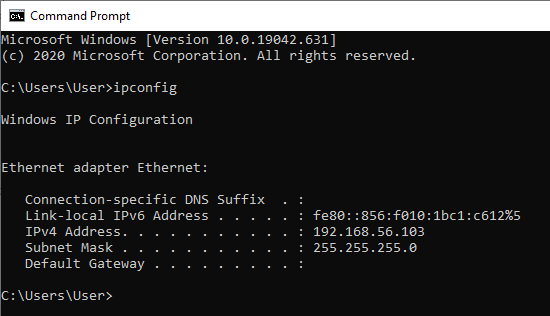
\includegraphics[width=\linewidth]{figures/target_ip.png}
    \caption{IP address of the target machine.}
    \label{fig:target-ip}
\end{figure}

\begin{figure}[H]
    \centering
    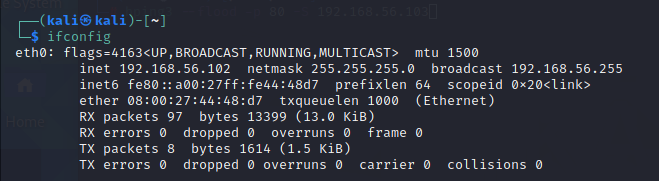
\includegraphics[width=\linewidth]{figures/attacker_ip.png}
    \caption{IP address of the attacking machine.}
    \label{fig:attack-ip}
\end{figure}

\begin{figure}[H]
    \centering
    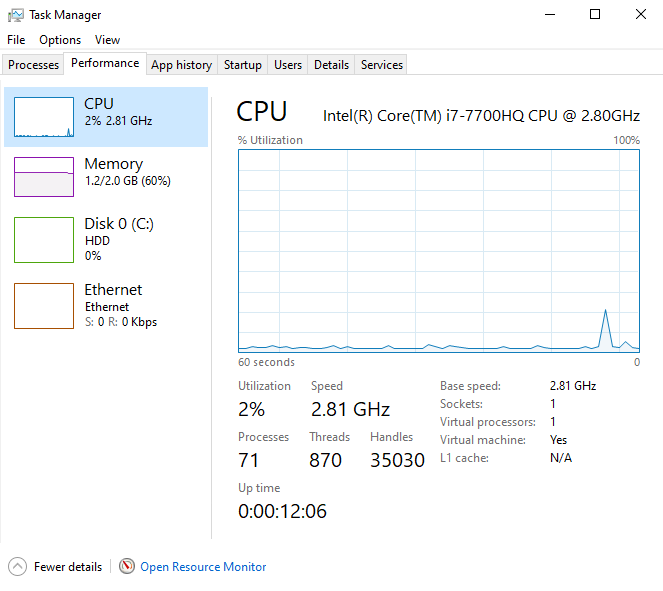
\includegraphics[]{figures/before_performance.png}
    \caption{Target machine performance before attack.}
    \label{fig:performance-before}
\end{figure}

\begin{figure}[H]
    \centering
    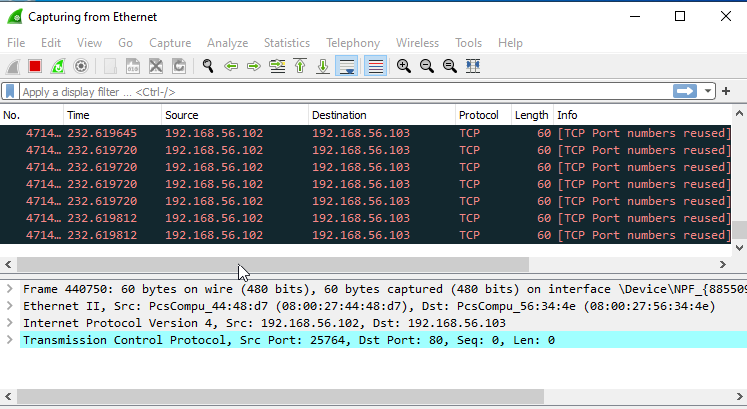
\includegraphics[width=\linewidth]{figures/target_packets.png}
    \caption{Packets being captured in Wireshark.}
    \label{fig:packets}
\end{figure}

\begin{figure}[H]
    \centering
    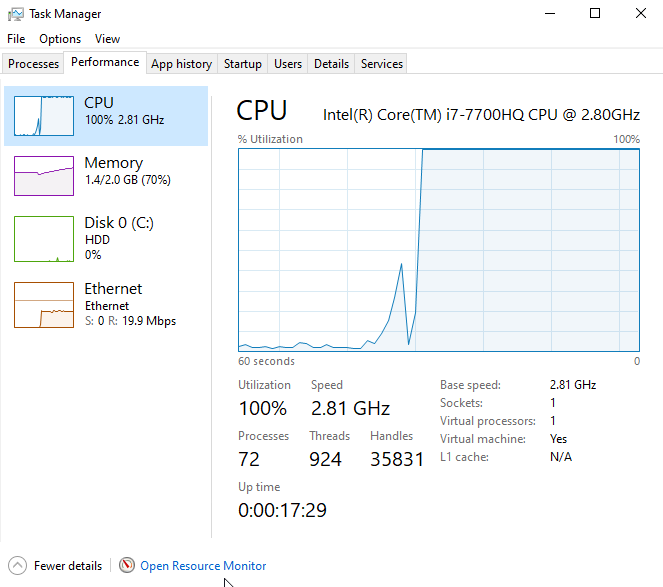
\includegraphics[width=\linewidth]{figures/during_performance.png}
    \caption{Target machine performance during the attack.}
    \label{fig:performance-during}
\end{figure}

\begin{figure}[H]
    \centering
    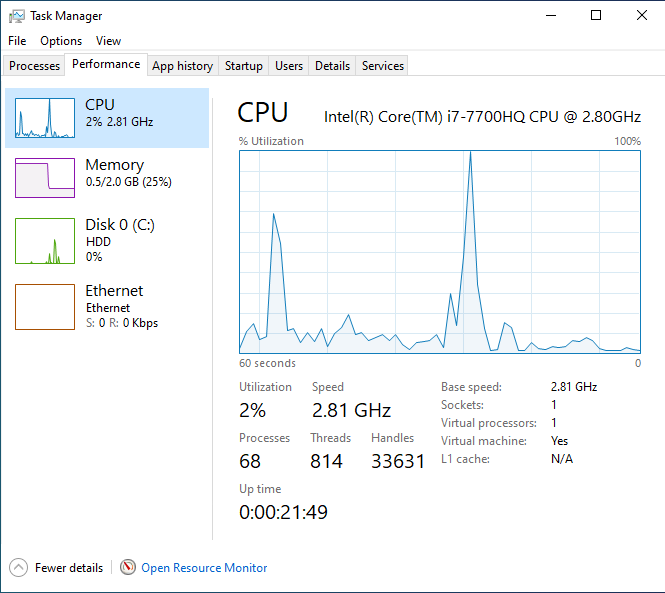
\includegraphics[width=\linewidth]{figures/after_performance.png}
    \caption{Target machine performance after the attack.}
    \label{fig:performance-after}
\end{figure}

\begin{figure}[H]
    \centering
    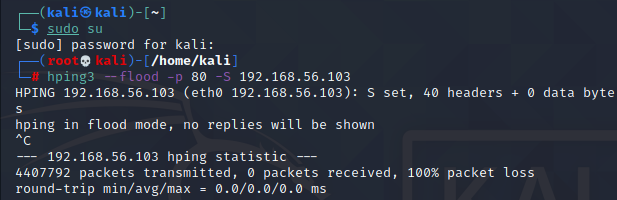
\includegraphics[width=\linewidth]{figures/hping_command.png}
    \caption{Hping3 command to create packets for address 192.168.56.103 port 80 with the SYN flag enabled.}
    \label{fig:hping}
\end{figure}

\newpage

Figure \ref{fig:performance-before} shows that there is minimal CPU and network usage before the attack, memory is at 60\% because there is not a lot of RAM allocated to the virtual machine.
Figure \ref{fig:packets} shows there is a large number of packets coming from \verb|192.168.56.102| (the attacker IP) to \verb|192.168.56.103| (the target IP).
In figure \ref{fig:performance-during} we see a spike in CPU, and Network usage, Memory usage seems to be ramping up as Wireshark collects packets.
Figures \ref{fig:performance-after} and \ref{fig:hping} show the aftermath of the attack, Network, CPU and Memory usage return to normal levels.
The result of the \verb|hping3| command show that there were over 4 million packets transferred.
DoS attacks can be very simple to initiate with the right tools and a list of IP addresses, and can cripple a network until the attacker decides to stop.
Firewalls and routers can block specific traffic associated with an attack (block the attacker IP address) but will not defend against an attacker spoofing a valid IP.